\section{Evaluation}
\label{sec:tern-evaluation}

Our \tern implementation consists of 8,934 lines of C++ code, including 827
lines for the instrumentor implemented as an LLVM pass; 5,451 lines for
the proxy, schedule cache, memoizer, and replayer; and 2,656 lines for
modifications to \klee.

We evaluated \tern on a diverse set of 14 programs, ranging from two server
programs, \apache and \mysql, to one parallel compression utility, \pbzip, to
11 scientific programs in \splash.\footnote{The version of the
  SPLASH2~\cite{lu:bugbench} we acquired has 12 programs, one of which does
  not compile on our evaluation machine.}
%  \pbzip and \splash programs are batch programs.
% Table~\ref{table:apps} column Size shows the size of these programs.  

Our main evaluation machine is a 2.66 GHz quad-core Intel machine with 4
GB memory running Linux 2.6.24.  When evaluating \tern on server programs, we
ran the server on this machine and the client on another to avoid
unnecessary contention.  These machines are connected via 1Gbps LAN.  We
compiled all programs down to machine code using \vv{llvm-gcc -O2} and
LLVM's bitcode compiler \vv{llc}.

We focused our evaluation on four key questions:
\begin{enumerate}

\item Is \tern easy to use (\S\ref{sec:tern-ease-of-use})?

\item Does \tern make multithreaded programs stable across different inputs
  (\S\ref{sec:tern-stability})?

\item Does \tern incur high overhead (\S\ref{sec:tern-overhead})?

\item Does \tern make multithreaded programs deterministic on the same
  input (\S\ref{sec:tern-determinism})?

\end{enumerate}


\subsection{Ease of Use}\label{sec:tern-ease-of-use}

\begin{table}
\centering
\footnotesize
\begin{tabular}{cccccc}
{\bf Program} & {\bf Size} & {\bf Symbolic} & {\bf Task} & {\bf Sync} & {\bf Total}\\
\hline
% -6.0 
\apache        & 464K   & 4  & 2   &  0  & 6 (+1) \\
\mysql         & 1,182K & 1  & 2   &  0  & 3 (+28) \\
\pbzip         & 1,551  & 3  & N/A &  0  & 3  \\
\fft           & 1,403  & 4  & N/A &  0  & 4  \\   
\lu            & 1,265  & 3  & N/A &  0  & 3  \\   
\barnes        & 1,954  & 9  & N/A &  0  & 9  \\
\radix         & 661    & 4  & N/A &  0  & 4  \\   
\fmm           & 3,208  & 8  & N/A &  1  & 9  \\   
\ocean         & 6,494  & 5  & N/A &  0  & 5  \\   
\volrend       & 18,082 & 1  & N/A &  1  & 2  \\   
\waters        & 1,573  & 9  & N/A &  0  & 9  \\   
\raytrace      & 5,808  & 3  & N/A &  0  & 3  \\   
\watern        & 1,188  & 10 & N/A &  0  & 10  \\   
\cholesky      & 3,683  & 3  & N/A &  1  & 4  \\
\end{tabular}
\caption{\small {\em Statistics of programs evaluated.} {\bf Size}
  counts the lines of code for each program.  {\bf Symbolic} counts the
  symbolic variables we marked.  {\bf Task} counts the task boundary
  annotations (\vv{begin\_task()} and \vv{end\_task()}) we inserted.  {\bf
    Sync} counts the annotations for custom synchronizations we inserted.
  The numbers in parenthesis under {\bf Total} count miscellaneous
  changes.} \label{table:tern-apps}
\end{table}

Table~\ref{table:tern-apps} summarizes the modifications we made to make the
programs work with \tern.  For each program but \mysql, we modified only 3-10
lines.  For \apache, we marked the HTTP command, URL, HTTP version, and the
return of \vv{cache\_find()} as symbolic (\S\ref{sec:tern-window}).  For \mysql,
we marked the SQL query.  For \pbzip, we marked the number of threads and
file blocks.  (The number of file blocks is set in two places,
contributing two symbolic annotations.)  For all these scientific programs, we
marked all input arguments as symbolic except those configuring output
verbosity.\footnote{Note that we could have used a two-line loop to mark
  these arguments as symbolic.  Instead, we report the total number of
  symbolic variables to avoid masking real data.}  We marked three custom
synchronization operations in three \splash programs.  We made two
miscellaneous changes to \apache and \mysql.  The line counts are shown in
parenthesis under the Total column.  For \apache, we had to fix an
uninitialized memory read in \vv{ap\_signal\_server()} to make it work with
\klee.  For \mysql, we wrote a 28-line function to mark the numbers in each
SQL query as concrete (\ie, not affecting schedules) to avoid making the
input constraints too specific.

\subsection{Stability} \label{sec:tern-stability}

We evaluated \tern's stability via two sets of experiments.  The first set
compares it to an existing \dmt system (\S\ref{sec:tern-bug-stable}). The
second quantifies how frequently it can reuse schedules on real and
synthetic workloads (\S\ref{sec:tern-reuse-rate}).

\subsubsection{Bug Stability} \label{sec:tern-bug-stable}

%%\newcommand{\bug}{\ding{54}\xspace}
%%\newcommand{\nobug}{\ding{52}\xspace}

\begin{table}
\small
\centering
\begin{tabular}{c|c@{\hspace{.07in}}cc
                 |c@{\hspace{.07in}}cc
                 |c@{\hspace{.07in}}cc}

{\bf      }& \multicolumn{3}{|c|}{\bf Nondet} 
           & \multicolumn{3}{|c|}{\bf \coredet} 
           & \multicolumn{3}{|c }{\bf \tern} \\
\hline
{\bf -p2} & \nobug & \nobug & \nobug
          & \nobug & \bug   & \nobug
          & \nobug & \nobug & \nobug  \\
{\bf -p4} & \nobug & \nobug & \nobug
          & \bug   & \bug   & \nobug
          & \nobug & \nobug & \nobug \\
{\bf -p8} & \nobug & \nobug & \nobug
          & \bug   & \bug   & \bug
          & \nobug & \nobug & \nobug \\
\hline
{\bf Args.}& {\bf -m10} & {\bf 12} & {\bf 14}
           & {\bf -m10} & {\bf 12} & {\bf 14}
           & {\bf -m10} & {\bf 12} & {\bf 14} \\
\end{tabular}
\caption{{\em Bug stability results on \splash \vv{fft}.}  The leftmost
  column and the bottommost row show the command line arguments.  Option
  {\bf -p} specifies the number of threads, and {\bf -m} the amount of
  computation (matrix size).  Symbol \bug indicates that the bug occured,
  and \nobug the bug never occured. }
\label{tab:tern-coredet}
\end{table}

We compared \tern to \coredet~\cite{coredet:asplos10} in terms of \emph{bug
  stability}: does a bug occur in one run but disappear in another when
the input varies slightly?  We ran three buggy
\splash programs, fft, lu, and barnes, in three modes: nondeterministic
execution (Nondet), with \coredet, and with \tern.  We varied their inputs by
varying the number of threads and the amount of computation.
For each program, execution mode, and input combination, we ran
the program 100 times, and recorded whether the corresponding bug occurred.

We present only the fft results; the results of the other programs are
similar.  Table~\ref{tab:tern-coredet} shows the buggy behaviors of fft.
  In nondeterministic mode, the bug never
occurred, despite that each run almost always yielded a new
synchronization order. With \coredet, slight changes in computation made the
bug occur or disappear.  With \tern, the bug never occurred, and
\tern reused only three schedules for all runs, one for each
thread count.  


\subsubsection{Reuse Rates} \label{sec:tern-reuse-rate}

We also quantified how frequently \tern could reuse schedules.
Specifically, we measured the overall reuse rate, defined as the number of
inputs processed using memoized schedules over the total number of inputs.
The higher the reuse rates, the more stable the programs become.  \tern had
nearly 100\% overall reuse rates for the scientific programs after a small
number of memoization runs.  Thus, we focused on \apache, \mysql, and \pbzip
in out experiments.

We used four workloads to evaluate overall reuse rates:

\begin{enumerate}

\item[{\bf Apache-CS}:] a real 4-day trace from the Columbia CS website
  with 122,000 HTTP requests.  We wrote a script to replay this trace at a
  rate of 100 concurrent requests per second.

\item[{\bf SysBench-simple}:] SysBench~\cite{sysbench} in simple mode.  This
  synthetic workload consists of random select queries.

%% The simple workload , and the advanced transaction workload randomly
%% selects, updates, deletes, and inserts records.  For Apache, we

\item[{\bf SysBench-tx}:] SysBench in transaction mode.  This synthetic
  workload consists of random select, update, delete, and insert queries.

\item[{\bf PBZip2-usr}:] a random selection of 10,000 files from \vv{/usr}
  on our evaluation machine.

\end{enumerate}

For each workload, we first randomly selected 1\%-3\% of the workload and
ran the memoizer to populate the schedule cache.  We then ran the entire
workload with the replayer and measured the overall reuse rates.  We ran
eight worker threads for each program because they performed best (with or
without \tern) with this setting.

\begin{table}[t]
\centering
\begin{tabular}{lcc}
\small
{\bf Program-Workload} & {\bf Reuse Rates (\%)} & {\bf Schedules} \\
\hline
Apache-CS              &    90.3\%    &    100      \\
SysBench-simple        &   94.0\%    &    50      \\
SysBench-tx            &   44.2\%    &    109      \\
\pbzip-usr             &   96.2\%    &    90      \\
\end{tabular}
\caption{\small{\em \tern stability.} Column {\bf Schedules} indicates the number
  of schedules in the schedule cache.}
\label{tab:tern-stability}
\end{table}

Table~\ref{tab:tern-stability} shows the results.  For three out of the four
workloads, \tern could reuse a small number of schedules to process over
90\% of the inputs.  For MySQL-tx, \tern had a lower overall reuse rate.
The reasons are two fold.  First, this workload makes it unlikely to reuse
schedules because it mixes many randomly generated queries with different
types and parameters.  Second, we annotated only the SQL command as
symbolic without exposing the hidden states of \mysql (\S\ref{sec:tern-window})
so that we could measure \tern's performance in an adversarial setting.
Nonetheless, \tern managed to process 44.2\% of inputs with a small number
of schedules.




\subsection{Overhead} \label{sec:tern-overhead}

We used the following workloads to evaluate \tern's overhead.  For \apache, we
used ApacheBench~\cite{apachebench} to repeatedly download a 50KB webpage.
For \mysql, we used the SysBench-simple workload from the  previous subsection.
Both ApacheBench and SysBench are used by the server developers themselves.
We made these benchmarks CPU bound by fitting the web or
database in memory and by connecting the server and client via a 1 Gbps
LAN.  For \pbzip, we decompressed a 10 MB file.  For \splash programs, we
ran them typically for 10-100 ms.  We measured the execution time for
batch programs and the throughput (TPUT) and response time (RESP) for
server programs.  All numbers reported in this section were averaged over
50 runs.


\begin{figure}[t]
\centering
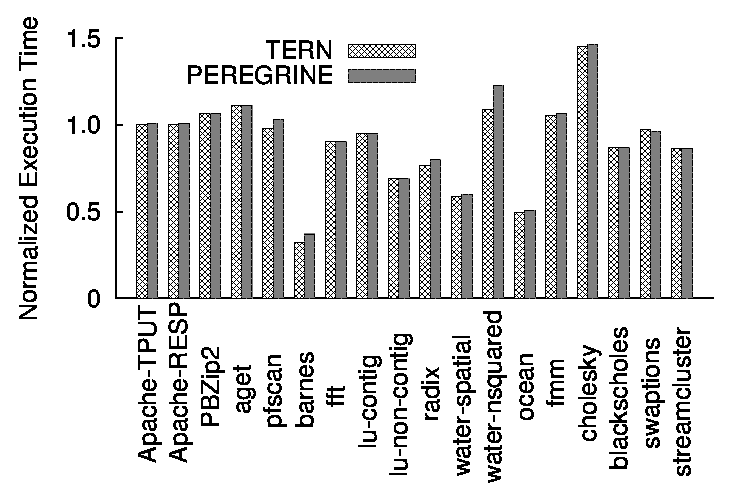
\includegraphics[width=0.5\textwidth]{tern/figures/overhead}

\caption{\small {\em Relative overhead of the replayer over
    nondeterministic execution.} Negative overhead means speedup.}
\label{fig:tern-overhead}
\end{figure}


The most performance-critical component is the replayer because it
operates during the normal execution of a program.
Figure~\ref{fig:tern-overhead} shows the relative overhead of the replayer over
nondeterministic execution, the smaller the better.  For seven out of
the fourteen programs, the replayer performed almost identically to
nondeterministic execution. For \pbzip and barnes, \tern performed
better.  This speedup came partially from the optimization to remove
unnecessary synchronizations, discussed in the next paragraph.  \tern's overhead
for \mysql, volrend, raytrace, water-nsquared, and choleskey is relatively
large because these programs performed many synchronization operations
over a short period of time.  For instance, water-nsquared and cholesky
both call \vv{pthread\_mutex\_lock()} and \vv{pthread\_mutex\_unlock()} in a
tight loop.


\begin{figure}[t]
\centering
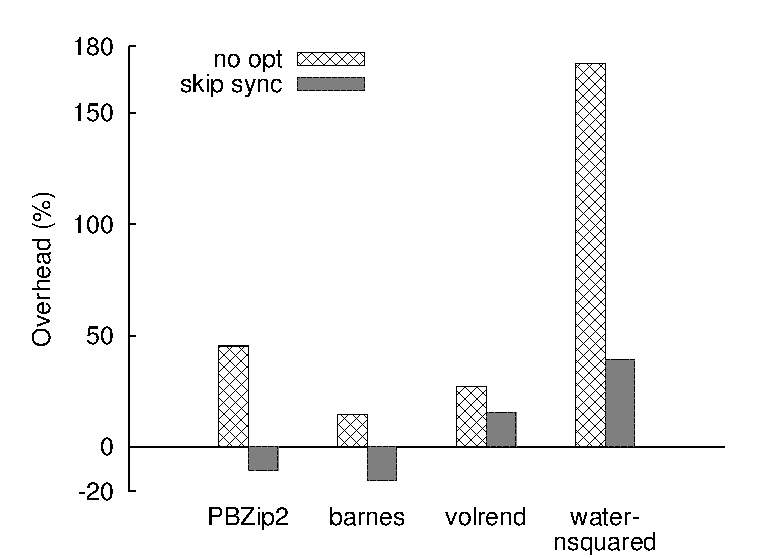
\includegraphics[width=0.5\textwidth]{tern/figures/opt-overhead}
\caption{\small {\em Overhead reduction by skipping unnecessary
    synchronizations.} ``no opt'' indicates the baseline overhead.}
\label{fig:tern-opt-remove-sync}
\end{figure}

We also measured the effects of skipping unnecessary synchronizations
(\S\ref{sec:tern-skip-waits}).  Figure~\ref{fig:tern-opt-remove-sync} shows the
results.  This optimization significantly reduced the replayer's overhead
for four programs.  Specifically, it made \pbzip and barnes run faster
than nondeterministic execution, and reduced the overhead of
water-nsquared from 172.4\% to 39.1\%.  Its effects on the other programs are
negligible and thus not shown.

\begin{figure}[t]
\centering
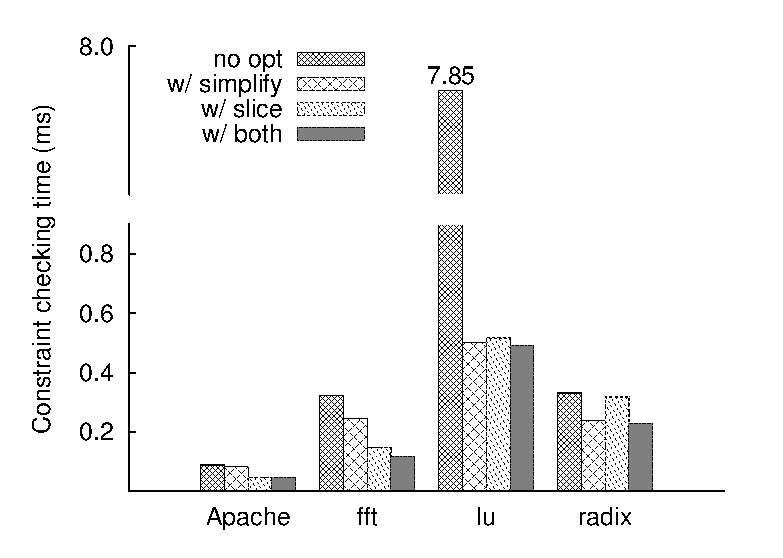
\includegraphics[width=0.5\textwidth]{tern/figures/expr-opt-time}
\caption{\small {\em Optimizations to speed up constraint checking.} Note
  the y-axis is broken. ``no opt'' indicates the baseline constraint checking
  time. ``simplify'' refers to the optimization in
  \S\ref{sec:tern-simplify}. ``slice'' refers to the optimization in
  \S\ref{sec:tern-slicing}.}
\label{fig:tern-opt-remove-constraints}
\end{figure}

\begin{table}[t]
\centering
\footnotesize
\begin{tabular}{lcccc}
{\bf Program} &  {\bf Nondet} &  {\bf Memoization} &  {\bf Overhead (times)}\\
\hline
Apache-TPUT   & 462.2 req/s         & 2.1 req/s                &   219.1\\
Apache-RESP   & 0.22 s        & 3.96 s            &   17.0\\
MySQL-TPUT    & 13779.3 req/s      & 172.2 req/s             &   79.0\\
MySQL-RESP    & 0.6 ms       & 61 ms             &   100.6\\
\pbzip        & 0.18 s        & 15.19 s           &   83.4\\
\end{tabular}
\caption{\small{\em Overhead of the memoizer.}}
\label{tab:tern-memoization-overhead}
\end{table}

To reuse a schedule on an input, \tern must check the input against
memoized constraints.  Constraint checking can be costly, and \tern provides
two optimizations to speed it up (\S\ref{sec:tern-simplify} and
\S\ref{sec:tern-slicing}).  Figure~\ref{fig:tern-opt-remove-constraints} shows these
optimizations can effectively speed up constraint checking for \apache,
fft, lu, and radix.  In particular, they reduced the constraint checking
time for lu by 16x.



Compared to the replayer, the memoizer can run offline, thus its
performance is not as critical.  Table~\ref{tab:tern-memoization-overhead}
shows that this slowdown can sometimes exceed 200x.  The main reason
is that \klee, the symbolic engine used, interprets programs instead of
running them natively.  An instrumentation-based approach can greatly
reduce this slowdown~\cite{cadar:exe:ccs06}, which we plan to implement in
our future work.  



\subsection{Determinism}\label{sec:tern-determinism}

We evaluated \tern's determinism via three sets of experiments.  The first
set checked the memoized schedules for races (\S\ref{sec:tern-race-results}).
The second evaluated \tern's ability to deterministically reproduce or avoid
bugs (\S\ref{sec:tern-bug-determinism}).  The third measured how deterministic
memory accesses are with and without
\tern (\S\ref{sec:tern-memory-determinism}).

\subsubsection{Race Detection Results}\label{sec:tern-race-results}

When memoizing schedules for each of the 14 programs, we turned on \tern's
race detector.  We found that except for radix and cholesky, the schedules
\tern memoized for all other programs were free of schedule races and
symbolic races with respect to the symbolic data we annotated
(\S\ref{sec:tern-detect-race}).  Our race detection result is not surprising
because most schedules are indeed race free.  It implies that, for runs
that reuse the memoized schedules of all programs but radix and cholesky,
\tern ensures determinism, barring the assumption discussed in
\S\ref{sec:tern-detect-race}.

\subsubsection{Bug Determinism}\label{sec:tern-bug-determinism}

%\hspace{-.1in}
\begin{table}[t]
\begin{center}
{
\small
\begin{tabular}{lp{2.3in}}

{\bf Program} & {\bf Error Description} \\

\hline

\apache & Reference count decrement and check against 0 are not atomic.\\

\pbzip & Variable \vv{fifo} is used in one thread after being freed by another.\\


fft & \vv{initdonetime} and  \vv{finishtime} are read
before assigned the correct values.\\

lu & Variable \vv{rf} is read before assigned the  correct
value. \\

barnes & Variable \vv{tracktime} is read before assigned the
correct value.\\

\end{tabular}}
\end{center}
\caption{{\em Concurrency errors used in evaluation}.} \label{table:tern-races}
\end{table}

We also evaluated how deterministically \tern could reproduce or avoid
bugs.  Table~\ref{table:tern-races} lists five real concurrency bugs we used.
We selected them because they were frequently used in previous
studies~\cite{avio:asplos06,ctrigger:asplos09,lu:concurrency-bugs,pres:sosp09}
and we could reproduce them on our evaluation machine.  To measure bug
determinism, we first memoized schedules for programs listed in
Table~\ref{table:tern-races}.  We then manually inserted \vv{usleep()} to these
programs to get alternate schedules.  We then ran the buggy programs
again, reusing the memoized schedules.  We also injected random delays
into the reuse runs to perturb timing.  We found that, \tern consistently
reproduced or avoided all five bugs.  We verified this result
by inspecting the memoized schedules.

\subsubsection{Memory Access Determinism}\label{sec:tern-memory-determinism}

\tern enforces synchronization orders, which should make memory access
orders more deterministic.  We quantified this effect over \apache and
\pbzip.  Specifically, we instrumented \apache with LLVM to trace accesses
to global variables and the heap, a crude approximation of shared memory.
We ran \apache with \tern to serve five HTTP requests and collected a trace
of memory accesses.  We then repeated this experiment 20 times to collect
20 traces, and computed the average pairwise edit
distance~\cite{edit-distance}.  We then measured the same edit distance
for \apache in nondeterministic execution mode and compared the two.  We
did the same comparison for \pbzip with a decompression workload of 2MB.  
Table~\ref{tab:tern-memory-determinism} shows the result.  For \apache,
runs with \tern were 7.97 times more deterministic than those without.  For
\pbzip, \tern was 2.33 times more deterministic, but the memory trace had
only 1,234 accesses on average.


\begin{table}
\centering
\small
\begin{tabular}{ccccc}
{\bf Program} & {\bf Length} & {\bf Nondet} & {\tern} & {\bf Ratio} \\
\hline
\apache & 148,058 & 86,215 & 10,821 & 7.97 \\
\pbzip & 1,234   & 161   & 69    & 2.33 \\
\end{tabular}
\caption{\small{\em Memory access determinism.}  We traced memory accessed
  only from \pbzip, not the external BZip2
  library.} \label{tab:tern-memory-determinism}
\end{table}






